\documentclass[border=3pt,tikz]{standalone}
% Gemeinsame Praeambel aller Abbildungen — Palette und Styles identisch zum
% GermEval-2026-Paper (Nuernberg NLP), damit die Bilder dort wiederverwendbar
% sind, ohne neu gezeichnet zu werden.
\usepackage{xcolor}
\usepackage{ifthen}
\usepackage{tikz}
\usetikzlibrary{shapes,arrows.meta,positioning,fit,backgrounds,calc,decorations.pathreplacing}

\definecolor{clrPrompt}{HTML}{B0CA97} % green  — Prompting (baseline)
\definecolor{clrSFT}{HTML}{E8A087}    % salmon — SFT (generative)
\definecolor{clrCls}{HTML}{88C4C8}    % teal   — ClsHead / FT (discriminative)
\definecolor{clrEns}{HTML}{D1BC8A}    % gold   — ensemble / majority vote
\definecolor{clrPCS}{HTML}{B7A0C9}    % purple — minority-class scope
\definecolor{clrBase}{HTML}{9AA0A6}   % grey   — untrained/frozen base

\tikzset{
  sysbox/.style={rectangle, rounded corners=3pt, line width=0.9pt,
    minimum width=2.7cm, minimum height=0.82cm, align=center,
    inner ysep=2pt, inner xsep=4pt, font=\fontsize{7.5}{9}\selectfont\bfseries},
  voterchip/.style={rectangle, rounded corners=1.5pt, line width=0.55pt,
    minimum width=0.78cm, minimum height=0.36cm, align=center,
    inner sep=1pt, font=\fontsize{5.4}{6.4}\selectfont},
  major/.style={rectangle, rounded corners=3pt, line width=0.9pt,
    align=center, font=\footnotesize\bfseries, inner ysep=4pt, inner xsep=10pt},
  io/.style={rectangle, rounded corners=2pt, line width=0.55pt, align=center,
    minimum width=1.35cm, minimum height=0.72cm, fill=black!3, draw=black!35,
    font=\fontsize{7.2}{8.6}\selectfont},
  bb/.style={rectangle, rounded corners=3pt, line width=0.8pt, align=center,
    minimum width=2.35cm, minimum height=0.86cm,
    font=\fontsize{7.4}{8.8}\selectfont},
  lab/.style={rectangle, rounded corners=1.2pt, line width=0.45pt,
    minimum height=0.30cm, align=center, inner sep=1.5pt,
    font=\fontsize{5.6}{6.8}\selectfont},
  edge/.style={-{Stealth[length=4pt]}, line width=0.6pt, black!50},
  bus/.style={line width=0.6pt, black!50},
  note/.style={font=\fontsize{6.4}{7.8}\selectfont\itshape, text=black!55,
    align=center},
  hdr/.style={font=\fontsize{6.5}{8}\selectfont\bfseries, text=black!55},
}

\begin{document}
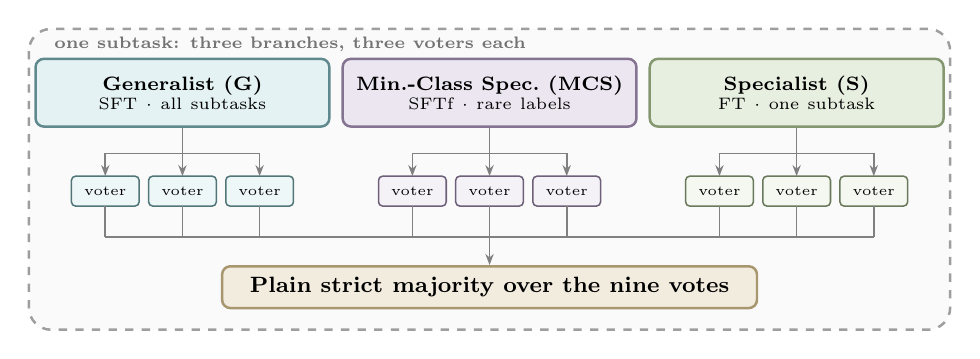
\begin{tikzpicture}[
  branchbox/.style={sysbox, text width=3.45cm, minimum width=3.65cm,
    minimum height=0.86cm, font=\fontsize{6.9}{8.4}\selectfont\bfseries},
  chip/.style={voterchip, minimum width=0.86cm, minimum height=0.38cm},
]

\def\ybox{1.05}    % Mitte der Branch-Box
\def\ybus{0.28}    % Verteiler unter der Box
\def\ychip{-0.20}  % Mitte der Voter-Chips
\def\ycol{-0.78}   % Sammelschiene
\def\yens{-1.42}   % Mehrheitsbalken

\def\cA{-3.90}
\def\cB{0}
\def\cC{3.90}
\def\dchip{0.98}

\begin{scope}[on background layer]
  \draw[draw=black!38, dashed, rounded corners=8pt, line width=0.9pt,
        fill=black!2] (-5.85, 1.86) rectangle (5.85, -1.96);
\end{scope}
\node[hdr, anchor=west] at (-5.65, 1.66)
  {\textsc{one subtask: three branches, three voters each}};

\node[branchbox, draw=clrCls!70!black, fill=clrCls!22] (bA) at (\cA, \ybox)
  {Generalist (G)\\[-1.5pt]{\fontsize{5.8}{7}\selectfont\mdseries
   SFT $\cdot$ all subtasks}};
\node[branchbox, draw=clrPCS!72!black, fill=clrPCS!26] (bB) at (\cB, \ybox)
  {Min.-Class Spec.\ (MCS)\\[-1.5pt]{\fontsize{5.8}{7}\selectfont\mdseries
   SFTf $\cdot$ rare labels}};
\node[branchbox, draw=clrPrompt!75!black, fill=clrPrompt!30] (bC) at (\cC, \ybox)
  {Specialist (S)\\[-1.5pt]{\fontsize{5.8}{7}\selectfont\mdseries
   FT $\cdot$ one subtask}};

% Jede Verbindung: senkrecht auf den Verteiler, waagerecht, senkrecht in den
% Chip, senkrecht weiter auf die Sammelschiene. Keine Diagonalen, alle drei
% Branches identisch aufgebaut.
\foreach \bb/\xc/\clr in {bA/\cA/clrCls, bB/\cB/clrPCS, bC/\cC/clrPrompt}{
  \draw[bus] (\bb.south) -- (\xc, \ybus);
  \draw[bus] ({\xc-\dchip}, \ybus) -- ({\xc+\dchip}, \ybus);
  \foreach \dx in {-\dchip, 0, \dchip}{
    \node[chip, draw=\clr!60!black, fill=\clr!14] at ({\xc+\dx}, \ychip) {voter};
    \draw[edge] ({\xc+\dx}, \ybus) -- ({\xc+\dx}, {\ychip+0.19});
    \draw[bus]  ({\xc+\dx}, {\ychip-0.19}) -- ({\xc+\dx}, \ycol);
  }
}

\draw[bus] ({\cA-\dchip}, \ycol) -- ({\cC+\dchip}, \ycol);
\node[major, draw=clrEns!80!black, fill=clrEns!28] (ens) at (0, \yens)
  {Plain strict majority over the nine votes};
\draw[edge] (0, \ycol) -- (ens.north);

\end{tikzpicture}
\end{document}
